% v2-acmsmall-sample.tex, dated March 6 2012
% This is a sample file for ACM small trim journals
%
% Compilation using 'acmsmall.cls' - version 1.3 (March 2012), Aptara Inc.
% (c) 2010 Association for Computing Machinery (ACM)
%
% Questions/Suggestions/Feedback should be addressed to => "acmtexsupport@aptaracorp.com".
% Users can also go through the FAQs available on the journal's submission webpage.
%
% Steps to compile: latex, bibtex, latex latex
%
% For tracking purposes => this is v1.3 - March 2012

\documentclass[prodmode,acmtecs]{acmsmall} % Aptara syntax

\usepackage{graphicx}
\usepackage{caption}
\usepackage{subfigure}
\usepackage{setspace}
\usepackage{tabulary}
\usepackage{fancybox}

% font in listings
\usepackage{courier}

\makeatletter
\newenvironment{CenteredBox}{% 
\begin{Sbox}}{% Save the content in a box
\end{Sbox}\centerline{\parbox{\wd\@Sbox}{\TheSbox}}}% And output it centered
\makeatother

\let\proof\relax
\let\endproof\relax
\usepackage{amsthm}
\newcommand{\specialcell}[2][c]{%
  \begin{tabular}[#1]{@{}c@{}}#2\end{tabular}}

\usepackage{lineno}
\usepackage{xfrac}

% Theorems, definitions, lemmas, etc
\newtheorem{Def}{Definition}
\newtheorem{Prop}{Proposition}
\newtheorem*{Rem*}{Remark}

\usepackage{alltt}
\renewcommand{\ttdefault}{txtt}

\usepackage{listings}
\lstset{language=C, breaklines=true, mathescape}

\usepackage[cmex10]{amsmath}
\usepackage{url}



% Metadata Information
%\acmVolume{9}
%\acmNumber{4}
%\acmArticle{39}
%\acmYear{2010}
%\acmMonth{3}

% Document starts
\begin{document}

% Page heads
\markboth{F. Luporini et al.}{On Optimality of Finite Element Integration}

% Title portion
\title{On Optimality of Finite Element Integration}
\author{Fabio Luporini
\affil{Imperial College London}
David A. Ham
\affil{Imperial College London}
Paul H.J. Kelly
\affil{Imperial College London}}

\begin{abstract}
We tackle the problem of automatically generating optimal finite element integration routines given a high level specification of arbitrary multilinear forms. Optimality is defined in terms of floating point operations required to execute a loop nest. The generation of optimal loop nests is driven by a model that exploits mathematical properties of the domain of interest. A theoretical analysis and extensive experimentation prove the effectiveness of our approach, showing systematic performance improvements over a number of alternative code generation systems. The effect of low-level optimization is also discussed.
\end{abstract}

\category{G.1.8}{Numerical Analysis}{Partial Differential Equations -
  Finite element methods}

\category{G.4}{Mathematical Software}{Parallel and vector implementations}

\terms{Design, Performance}

\keywords{Finite element integration, local assembly, compilers, performance optimization}

\acmformat{Fabio Luporini, David A. Ham, and Paul   H. J. Kelly, 2015. On Optimality of Finite Element Integration.}

% At a minimum you need to supply the author names, year and a title.
% IMPORTANT: Full first names whenever they are known, surname last,
% followed by a period.  In the case of two authors, 'and' is placed
% between them.  In the case of three or more authors, the serial
% comma is used, that is, all author names except the last one but
% including the penultimate author's name are followed by a comma, and
% then 'and' is placed before the final author's name.  If only first
% and middle initials are known, then each initial is followed by a
% period and they are separated by a space.  The remaining information
% (journal title, volume, article number, date, etc.) is
% 'auto-generated'.

\begin{bottomstuff}

This research is partly funded by the MAPDES project, by the
Department of Computing at Imperial College London, by EPSRC through
grants EP/I00677X/1, EP/I006761/1, and EP/L000407/1, by NERC grants
NE/K008951/1 and NE/K006789/1, by the U.S.  National Science
Foundation through grants 0811457 and 0926687, by the U.S. Army
through contract W911NF-10-1-000, and by a HiPEAC collaboration
grant. The authors would like to thank Mr. Andrew T.T. McRae,
Dr. Lawrence Mitchell, and Dr. Francis Russell for their invaluable
suggestions and their contribution to the Firedrake project.

Author's addresses: Fabio Luporini $\&$ Paul H. J. Kelly, Department of Computing,
Imperial College London; David A. Ham, Department of Computing and
Department of Mathematics, Imperial College London; 
\end{bottomstuff}

\maketitle


\section{Introduction}

The need for rapidly implementing high performance, robust, and portable finite element methods has led to approaches based on automated code generation. This has been proved successful in the context of the FEniCS (\cite{Fenics}) and Firedrake (\cite{firedrake-code}) projects, which have become increasingly popular over the last years. In these frameworks, the weak variational form of a problem is expressed at high-level by means of a domain-specific language. The mathematical specification is manipulated by a form compiler that generates a representation of assembly operators. By applying these operators to an element in the discretized domain, a local matrix and a local vector, which represent the contributions of that element to the equation solution, are computed. The code for assembly operators should be high performance: as the complexity of a variational form increases, in terms of number of derivatives, pre-multiplying functions, or polynomial order of the chosen function spaces, the operation count increases, with the result that assembly often accounts for a significant fraction of the overall runtime. 

As demonstrated by the considerable body of research on the topic, automating the generation of such high performance implementations poses several challenges. This is a result of the complexity inherent to the mathematical expressions involved in the numerical integration, which varies from problem to problem, and the particular structure of the loop nests enclosing the integrals. General-purpose compilers, such as \emph{GNU's} and \emph{Intel's}, fail at exploiting the structure inherent in the expressions, thus producing sub-optimal code (i.e., code which performs more floating-point operations, or ``flops'', than necessary). Research compilers, for instance those based on polyhedral analysis of loop nests such as PLUTO (\cite{PLUTO}), focus on parallelization and loop optimization for cache locality, so they are not particularly helpful in our context. The lack of suitable third-party tools has led to the development of a number of domain-specific code transformation (or synthesizer) systems. In~\citeN{quadrature1}, it is shown how automated code generation can be leveraged to introduce optimizations that a user should not be expected to write ``by hand''. In~\citeN{FFC-TC} and~\citeN{Francis}, mathematical reformulations of finite element integration are studied with the aim of minimizing the operation count. In~\citeN{Luporini}, the effects and the interplay of generalized code motion and a set of low-level optimizations are analysed. It is also worth mentioning an on-going effort to produce a novel form compiler, called UFLACS (\cite{Uflacs}), which adds to the already abundant set of code transformation systems for assembly operators. 

However, in spite of such a considerable research effort, still there is no answer to one fundamental question: can we automatically generate an implementation of a form which is optimal in the number of flops executed? In this paper, we formulate an approach to solve this problem. Summarizing, our contributions are as follows

\begin{itemize}
\item We characterize loop nest optimality and we instantiate this concept to finite element integration. As part of this construction, we establish the notion of sharing and demonstrate that sharing can always be eradicated from the loop nests we are interested in.
\item We provide a model centred on sharing and other mathematical properties of our domain of interest; the model drives the translation of a monomial appearing in a form into optimal loop nests.
\item We comment on the cases in which such model does not lead to optimal loop nests. We will see that this might occur with particular forms that make extensive use of tensor algebra. We show, however, that our model still is capable of producing quasi-optimal loop nests.
\item We integrate the model with a compiler, COFFEE\footnote{COFFEE stands for COmpiler For Fast Expression Evaluation. The compiler is open-source and available at \url{https://github.com/coneoproject/COFFEE}}, which is in use in the Firedrake framework.
\item We experimentally evaluate using a broader suite of forms, discretizations, and code generation systems than has been used in prior research. This is essential to demonstrate that our optimality model holds in practice.
\end{itemize}

In addition, in order to place COFFEE on the same level of other code generation systems from the viewpoint of low-level optimization (which is essential for a fair performance comparison)

\begin{itemize}
\item We introduce an engine based on symbolic execution that allows skipping irrelevant floating point operations (e.g., those involving zero-valued quantities). We elaborate on the performance impact of this optimization, making a clear distinction between flop optimality and efficient code.
\end{itemize}


\section{Preliminaries}
\label{sec:background}
We review finite element integration using the same notation and examples adopted in~\citeN{quadrature1} and~\citeN{Francis}. 

We consider the weak formulation of a linear variational problem
\begin{equation}
\begin{split}
Find\ u\ \in U\ such\ that \\
a(u, v) = L(v), \forall v \in V
\end{split}
\end{equation}
where $a$ and $L$ are, respectively, a bilinear and a linear form. The set of \textit{trial} functions $U$ and the set of \textit{test} functions $V$ are discrete function spaces. For simplicity, we assume $U = V$. Let $\lbrace \phi_i \rbrace$ be the set of basis functions spanning $U$. The unknown solution $u$ can be approximated as a linear combination of the basis functions $\lbrace \phi_i \rbrace$. From the solution of the following linear system it is possible to determine a set of coefficients to express $u$:
\begin{equation}
A\textbf{u} = b
\end{equation}
in which $A$ and $b$ discretize $a$ and $L$ respectively:
\begin{equation}
\centering
\begin{split}
A_{ij} = a(\phi_i(x), \phi_j(x)) \\
b_i = L(\phi_i(x))
\end{split}
\end{equation}
The matrix $A$ and the vector $b$ are ``assembled'' and subsequently used to solve the linear system through (typically) an iterative method.

We focus on the assembly phase, which is often characterized as a two-step procedure: \textit{local} and \textit{global} assembly. Local assembly is the subject of this article. It consists of computing the contributions of a single element in the discretized domain to the equation solution. In global assembly, such local contributions are ``coupled'' by suitably inserting them into $A$ and $b$. 

We illustrate local assembly in a concrete example, the evaluation of the local element matrix for a Laplacian operator. Consider the weighted Laplace equation
\begin{equation}
- \nabla \cdot (w \nabla u) = 0
\end{equation}
in which $u$ is unknown, while $w$ is prescribed. The bilinear form associated with the weak variational form of the equation is:
\begin{equation}
a(v, u) = \int_\Omega w \nabla v \cdot \nabla u\ \mathrm{d}x
\end{equation}
The domain $\Omega$ of the equation is partitioned into a set of cells (elements) $T$ such that $\bigcup T = \Omega$ and $\bigcap T = \emptyset$. By defining $\lbrace \phi_i^K \rbrace$ as the set of local basis functions spanning $U$ on the element $K$, we can express the local element matrix as
\begin{equation}
\label{stiffness}
A_{ij}^K = \int_K w \nabla \phi_i^K \cdot \nabla \phi_j^K\ \mathrm{d}x
\end{equation}
The local element vector $L$ can be determined in an analogous way. 
%From the computational perspective, its evaluation is however less expensive than that of $A$.

\subsection{Quadrature Mode}
Quadrature schemes are typically used to numerically evaluate $A_{ij}^K$. For convenience, a reference element $K_0$ and an affine mapping $F_K : K_0 \rightarrow K$ to any element $K \in T$ are introduced. This implies that a change of variables from reference coordinates $X_0$ to real coordinates $x = F_K (X_0)$ is necessary any time a new element is evaluated. The numerical integration routine based on quadrature over an element $K$ can be expressed as follows
\begin{equation}
\label{eq:quadrature}
A_{ij}^K = \sum_{q=1}^N \sum_{\alpha_3=1}^n \phi_{\alpha_3}(X^q)w_{\alpha_3} \sum_{\alpha_1=1}^d \sum_{\alpha_2=1}^d \sum_{\beta=1}^d \frac{\partial X_{\alpha_1}}{\partial x_{\beta}} \frac{\partial \phi_i^K(X^q)}{\partial X_{\alpha_1}} \frac{\partial X_{\alpha_2}}{\partial x_{\beta}} \frac{\partial \phi_j^K(X^q)}{\partial X_{\alpha_2}} det F_K' W^q
\end{equation}
where $N$ is the number of integration points, $W^q$ the quadrature weight at the integration point $X^q$, $d$ is the dimension of $\Omega$, $n$ the number of degrees of freedom associated to the local basis functions, and $det$ the determinant of the Jacobian matrix used for the aforementioned change of coordinates.  

% Magari la summation sui coefficients la sputo dentro? che dici?

\subsection{Tensor Contraction Mode}
Starting from Equation~\ref{eq:quadrature}, exploiting linearity, associativity and distributivity of the involved mathematical operators, we can rewrite the expression as
\begin{equation}
\label{eq:tensor}
A_{ij}^K = \sum_{\alpha_1=1}^d \sum_{\alpha_2=1}^d \sum_{\alpha_3=1}^n det F_K' w_{\alpha_3} \sum_{\beta=1}^d \frac{X_{\alpha_1}}{\partial x_{\beta}} \frac{\partial X_{\alpha_2}}{\partial x_{\beta}} \int_{K_0} \phi_{\alpha_3} \frac{\partial \phi_{i_1}}{\partial X_{\alpha_1}} \frac{\partial \phi_{i_2}}{\partial X_{\alpha_2}} dX.
\end{equation}
A generalization of this transformation has been proposed in~\cite{Kirby:TC}. By only involving reference element terms, the integral in the equation can be pre-evaluated and stored in temporary variables. The evaluation of the local tensor can then be abstracted as
\begin{equation}
A_{ij}^K = \sum_{\alpha} A_{i_1 i_2 \alpha}^0 G_{K}^\alpha
\end{equation}
in which the pre-evaluated ``reference tensor'' $A_{i_1 i_2 \alpha}$ and the cell-dependent ``geometry tensor'' $G_{K}^\alpha$ are exposed. 

\subsection{Qualitative Comparison}
\label{sec:qualitative}
Depending on form and discretization, the relative performance of the two modes, in terms of the operation count, can vary quite dramatically. The presence of derivatives or coefficient functions in the input form tends to increase the size of the geometry tensor, making the traditional quadrature mode preferable for ``complex'' forms. On the other hand, speed-ups from adopting tensor mode can be significant in a wide class of forms in which the geometry tensor remains ``sufficiently small''. The discretization, particularly the relative polynomial order of trial, test, and coefficient functions, also plays a key role in the resulting operation count. 

These two modes have been implemented in the FEniCS Form Compiler (\cite{FFC-TC}). In this compiler, a heuristic is used to choose the most suitable mode for a given form. It consists of analysing each monomial in the form, counting the number of derivatives and coefficient functions, and checking if this number is greater than a constant found empirically (\cite{Fenics}). We will later comment on the efficacy of this approach (Section~\ref{sec:optimal-synthesis}. For the moment, we just recall that one of the goals of this research is to produce an intelligent system that goes beyond the dichotomy between quadrature and tensor modes. We will reason in terms of loop nests, code motion, and code pre-evaluation, searching the entire implementation space for an optimal synthesis.  

\section{Problem Characterization}
\label{sec:optimal-impl}

In this section, we characterize optimality for finite element integration and the loop transformation space that we need to explore to achieve it. 

\subsection{Loop Nests and Optimality}
In order to make the document self-contained, we start with reviewing basic compiler terminology.

\begin{Def}[Perfect and imperfect loop nests]
A perfect loop nest is a loop whose body either 1) comprises only a sequence
of non-loop statements or 2) is itself a perfect loop nest. If this
condition does not hold, a loop nest is said to be imperfect. 
\end{Def}

\begin{Def}[Independent basic block]
An independent basic block is a sequence of statements such that no data
dependencies exist between statements in the block.
\end{Def}

We focus on perfect nests whose innermost loop body is an independent basic
block. A straightforward property of this class is that hoisting invariant
expressions from the innermost to any of the outer loops or the preheader
(i.e., the block that precedes the entry point of the nest) is always safe,
as long as any dependencies on loop indices are honored. We will make use of this property. The results of this section could also be generalized to larger classes of loop nests, in which basic block independence does not hold, although this would require refinements beyond the scope of this paper. 

By mapping mathematical properties to the loop nest level, we introduce the
concepts of a \textit{linear loop} and, more generally, a (perfect) multilinear loop nest.

\begin{Def}[Linear loop]
A loop $L$ defining the iteration space $I$ through the iteration variable $i$, or simply $L_i$, is \textit{linear} if 
\begin{enumerate}
\item $i$ appears in the body of $L$ only as an array index, and
\item whenever an array $a$ is indexed by $i$ ($a[i]$), all expressions in which this appears are affine in $a$.
\end{enumerate}
\end{Def}

\begin{Def}[Perfect multilinear loop nest]
A perfect multilinear loop nest of arity $n$ is a perfect nest composed of $n$ loops, in which all of the expressions appearing in the body of the innermost loop are linear in each loop $L_i$ separately.
\end{Def}

Since our focus is on finite element integration, for simplicity we restrict ourselves to the following, notable subclass of perfect multilinear loop nests.

\begin{Def}[Outer-product loop nest]
An outer-product loop nest is a perfect multilinear loop nest of arity $n \leq 2$ in which all of the expressions appearing in the body of the innermost loop are summations of outer products.
\end{Def}

As shown later, outer-product loop nests are important because they possess properties that we can take advantage of to synthesize optimal code. They arise naturally when translating bilinear or linear forms into code. Consider Equation~\ref{eq:quadrature} and the (abstract) loop nest implementing it illustrated in Figure~\ref{code:loopnest}. The imperfect nest $\Lambda=[L_e, L_i, L_j, L_k]$ comprises the element loop $L_e$, the integration loop $L_i$ (a reduction loop), and the outer-product loop nest $[L_j, L_k]$ over test and trial functions. The expression \texttt{F} implements the operator.

% (the Laplacian operator in the case of Equation~\ref{eq:quadrature}, but our discussion applies in general).
\begin{figure}[h]\begin{CenteredBox}
\lstinputlisting[basicstyle=\footnotesize\ttfamily]{listings/loopnest.code}
\end{CenteredBox}\caption{The typical loop nest implementing a bilinear form.}\label{code:loopnest}\end{figure}

Our aim is a strategy to synthesize optimal loop nests of this form. In particular, we characterize optimality as follows.

\begin{Def}[Optimality of a loop nest]
\label{def:mln-optimality}
Let $\Lambda$ be a generic loop nest, and let $\Gamma$ be a generic transformation function $\Gamma : \Lambda \rightarrow \Lambda'$ such that $\Lambda'$ is semantically equivalent to $\Lambda$ (possibly, $\Lambda' = \Lambda$). We say that $\Lambda' = \Gamma (\Lambda)$ is an optimal synthesis of $\Lambda$ if the number of operations that it performs to evaluate the result is minimal.
\end{Def}

Note that Definition~\ref{def:mln-optimality} does not take into account memory requirements. If the loop nest were memory-bound -- the ratio of operations to bytes transferred from memory to the CPU being too low -- then speaking of optimality would clearly make no sense. Henceforth we assume to operate in a CPU-bound regime, in which arithmetic-intensive expressions need be evaluated. In the context of finite element, this is often true for more complex multilinear forms and/or higher order elements.

\subsection{Transformation Space}
To synthesize optimal implementations we need:
\begin{itemize}
\item a characterization of the transformation space for the class of loop nests considered
\item a cost model to select the optimal point in the transformation space
\end{itemize}
In this section, we construct the transformation space. We leave a few loose hands, which we progressively tie in Section~\ref{sec:optimal-synthesis}.

We start with introducing the fundamental notion of sharing.

\begin{Def}[Sharing]
A loop $L_i$ presents sharing if it contains at least one statement in which two (sub-)expressions depending on $i$ are symbolically identical.
\end{Def}

\begin{Def}[Sharing factor]
The sharing factor of a loop $L_i$, $L^{sf}_i$, is given by the cardinality of the set of symbols depending on $i$ (i.e., arrays indexed by $i$). It provides an intuition of how many symbols can ideally be factored along $L_i$.
\end{Def}

\begin{figure}[h]\begin{CenteredBox}
{\subfigcapskip = 7pt \subfigure[With sharing]{\label{code:multi_loopnest_a}\lstinputlisting[basicstyle=\footnotesize\ttfamily]{listings/multilinear_loopnest.code}}}
~~~~~~~~~~~~~~
{\subfigcapskip = 2pt \subfigure[Optimal form]{\label{code:multi_loopnest_b}\lstinputlisting[basicstyle=\footnotesize\ttfamily]{listings/multilinear_loopnest_opt.code}}}
\end{CenteredBox}\caption{A simple outer-product loop nest. Note that $L^{sf}_i = 2$ and $L^{sf}_j = 1$.}\end{figure}

Figure~\ref{code:multi_loopnest_a} shows an example of a trivial outer-product loop nest of arity $n=2$ with sharing along dimension $j$ induced by $b_j$. Figure~\ref{code:multi_loopnest_b} shows an optimal synthesis for the loop nest in Figure~\ref{code:multi_loopnest_a}. More in general, arbitrarily complex outer-product loop nests can systematically be reduced to optimal form. The constructive proof that we provide below focuses on outer-product loop nests of arity $n=2$ (for $n < 2$ the proof is trivial; for $n > 2$, as we elaborate later, a more general treatise would be required).

\begin{Prop}
\label{prop:optimal-mln}
Assume $\Lambda = [L_{i_{0}}, L_{i_{1}}]$ is an outer-product loop nest with the body of $L_{i_{1}}$ being an independent basic block. Then an optimal synthesis $\Lambda'$ can be determined by eliminating sharing from both loops, starting from the loop with smallest sharing factor.
\end{Prop}
\begin{proof}
The demonstration is by construction and exploits linearity. We start with ``flattening'' the expressions (e.g., by multiplication expansion) in the body of $L_{i_{1}}$; this exposes the space of all possible factorizations. The resulting expressions are summations of outer products (otherwise, the assumption of $\Lambda$ being an outer-product loop nest would trivially be contradicted).

We traverse the expression tree and determine the sharing factor of the two linear loops. We take the symbols depending on the loop with smallest sharing factor, $L_i$, and we incrementally factorize them. Due to linearity, each factored product $P$ only has one symbol depending on $L_i$, and this symbol is now unique in the expression. The other term in $P$, independent of $L_i$, is, by definition, loop-invariant, and therefore hoisted such that redundant computation is avoided. We repeat the same process for the symbols along the loop with higher sharing factor, $L_j$. The transformations are semantically correct: multilinearity ensures deterministic factorization; perfectness ensures safeness of hoisting (see~\citeN{Luporini} for more details about generalized code motion).

We now have to demonstrate that the chosen factorization strategy, based on sharing factors, leads to optimality. This reduces to prove that the two following facts are true (we do it by contradiction).
\begin{enumerate}
\item Taking $L_j$, the loop with higher sharing factor, as point of departure would lead to a sub-optimal $\Lambda'$ (optimal only in the best case). If we assumed this were false, there would be two possibilities to consider: A) both $L_i$ and $L_j$ present sharing over disjoint sets of outer products; B) at least one outer product induces sharing along both $L_i$ and $L_j$. Case A) is quite trivial since there are no side effects in swapping the order of factorizations, so $\Lambda'$ would actually be optimal (best case scenario). In case B), due to linearity, factorization produces a summation of $L^{sf}_{j}$ outer products, as opposed to $L^{sf}_{i}$ if we had started with $L_i$. However, note that factorization followed by hoisting is always a winning strategy: evaluation, at every iteration, of hoisted symbols requires one operation (a sum) instead of the two operations (a product and a sum) needed by an outer product. Since $L^{sf}_{j} > L^{sf}_{i}$, it is clear that $\Lambda'$ could not be optimal, which contradicts the hypothesis.
\item Partial elimination of sharing would lead to a sub-optimal $\Lambda'$ (optimal only in the best case). Let us assume, for a moment, that this is false. In this scenario, at least one symbol is excluded from the factored product. Without loss of generality, consider, for instance, $a_i(b_j + c_j + ...) + a_i e_j + ...$. It is fairly obvious to see that either there is another factorization opportunity along $L_j$ ($e_j$ is shared with some other terms), in which case no additional operations need be performed, or $\Lambda'$ is sub-optimal. Consequently, the hypothesis is generally contradicted.
\end{enumerate}

Note that if we were considering outer-product loop nests of arity $n > 2$, unless relaxing Definition~\ref{def:mln-optimality}, we would need a much more complex construction to guarantee optimality. 
\end{proof}
  
We now observe that, for the larger class of finite element integration loop nests, the presence of sharing is a \textit{sufficient but not necessary} condition for being in \textit{non-optimal} form. Consider again the bilinear form implementation in Figure~\ref{code:loopnest}. We pose the following question: are we able to identify sub-expressions within $F$ for which the reduction imposed by $L_i$ can be pre-evaluated, thus obtaining a decrease in operation count proportional to the size of $L_i$, $M$? The transformation we look for is exemplified in Figures~\ref{code:loopnest_red} (input) and~\ref{code:loopnest_nored} (output); Figure~\ref{code:loopnest_red} can be seen as a simple instance of the abstract loop nest in Figure~\ref{code:loopnest}.

\begin{figure}[h]\begin{CenteredBox}
{\subfigcapskip = 19pt \subfigure[With reduction]{\label{code:loopnest_red}\lstinputlisting[basicstyle=\footnotesize\ttfamily]{listings/loopnest_red.code}}}
~~~~~~~~~~
{\subfigcapskip = 2pt \subfigure[Pre-evaluated reduction]{\label{code:loopnest_nored}\lstinputlisting[basicstyle=\footnotesize\ttfamily]{listings/loopnest_nored.code}}}
\end{CenteredBox}\caption{Exposition (through factorization) and pre-evaluation of a reduction.}\end{figure}

Pre-evaluation opportunities can be exposed through an exploration of the expression tree transformation space. For arbitrary loop nests, this can be challenging. Further, the following issues arise when considering pre-evaluation opportunities:
\begin{itemize}
\item as opposed to what happens with hoisting in outer-product loop nests, the temporary variable size is proportional to the number of non-reduction loops crossed (for the bilinear form implementation in Figure~\ref{code:loopnest}, $N \cdot O$ for sub-expressions depending on $[L_i, L_j, L_k]$ and $L \cdot N \cdot O$ for those depending on $[L_e, L_i, L_j, L_k] $). This might shift the loop nest from a CPU-bound to a memory-bound regime, which might be counter-productive for actual runtime
\item the transformations exposing pre-evaluation opportunities could increase the arithmetic complexity (e.g., expansion may increase the operation count; further examples will be provided later). This could overwhelm the gain inherent in pre-evaluation.
\end{itemize}

To summarize, so far we have highlighted four problems:
\begin{enumerate}
\item The need for an algorithm to expose pre-evaluation opportunities
\item Potential explosion in working set size
\item Potential increase in operation count due to manipulation of the expression tree
\item The need for a strategy to coordinate sharing elimination and pre-evaluation opportunities (sharing elimination could inhibit pre-evaluation; pre-evaluation might expose further sharing)
\end{enumerate}

We expand on these points in Section~\ref{sec:optimal-synthesis}. In the perspective of addressing point 2), we conclude this section refining our optimality statement as follows.

\begin{Def}[Optimality of a loop nest with bounded working set]
\label{def:optimality}
Let $\Lambda$ be a generic loop nest, and let $\Gamma$ be a generic transformation function $\Gamma : \Lambda \rightarrow \Lambda'$ such that $\Lambda'$ is semantically equivalent to $\Lambda$ (possibly, $\Lambda' = \Lambda$) and a set of memory constraints is satisfied. We say that $\Lambda' = \Gamma (\Lambda)$ is an optimal synthesis of $\Lambda$ if the number of operations that it performs to evaluate the result is minimal.
\end{Def}

\section{Transformation Algorithm}
\label{sec:optimal-synthesis}

In this section, we build a transformation algorithm capable of reducing finite element integration loop nests to optimal form. A fundamental aspect is the definition of a suitable cost function to assess the profitability of pre-evaluation (for which a deeper explanation will be provided). The optimality of the transformation algorithm is discussed.

\subsection{Memory constraints}
\label{sec:mem-const}
We provide intuitions about the need for memory constraints. Our point of departure is again the bilinear form implementation in Figure~\ref{code:loopnest}. Analogous considerations apply to forms of arbitrary arity.

The fact that $L \gg M, N, O$ suggests we should be cautious about hoisting mesh-dependent (i.e., $L_e$-dependent) expressions. Imagine $\Lambda$ is enclosed in a time stepping loop. One could think of exposing (through some transformations) and hoisting any time-invariant sub-expressions to minimize redundant computation at every time step. The working set size could then increase by a factor $L$. The gain in number of operations executed could therefore be overwhelmed, from a runtime viewpoint, by a much larger memory pressure.

A second, more general observation is that, for certain forms and discretizations, aggressive hoisting can make the working set exceed the size of ``some level of local memory'' (e.g. the last level of private cache on a conventional CPU, the shared memory on a GPU). For example, pre-evaluating geometry-independent expressions outside of $\Lambda$ requires temporary arrays of size $N\cdot O$ for bilinear forms and of size $N$ (or $O$) for linear forms. This can sometimes break such a ``local memory threshold''. In our experiments (Section~\ref{sec:perf-results-forms}) we will carefully study this aspect.

Based on these considerations, we establish the following set of memory constraints:
\begin{enumerate}
\item the size of a temporary due to code motion cannot be larger than that of the outer-product loop nest iteration space;
\item the total amount of memory occupied by the temporaries due to code motion cannot exceed a certain threshold, \texttt{$T_H$}.
\end{enumerate}
A corollary of constraint 1) is that hoisting expressions involving geometry-dependent terms outside of $\Lambda$, which is a possibility we discussed at the beginning of this section, is now forbidden. This clearly shrinks the transformation space, pruning points that most likely would result in sub-optimal performance.

\subsection{Reaching Optimality}
We here discuss how we can systematically reach the goal set by Definition~\ref{def:optimality}.

We reinforce the idea that eliminating sharing from the outer-product loop nest does not suffice. As suggested in Section~\ref{sec:optimal-impl}, we wonder whether, and under what conditions, the reduction imposed by $L_i$ could be pre-evaluated, thus reducing the operation count. 

To partly answer this question, we make use of a result -- the foundation of tensor contraction mode -- from~\citeN{Kirby:TC}. Essentially, multilinear forms can be seen as sums of monomials, each monomial being an integral over the equation domain of products (of derivatives) of functions from discrete spaces; such monomials can always be reduced to a product of two tensors (see Section~\ref{sec:background}). We interpret this result at the loop nest level: with an input as in Figure~\ref{code:loopnest}, we can always dissect \texttt{F} into distinct sub-expressions (the monomials). Each sub-expression is factorizable so as to split constants from $[L_i, L_j, L_k]$-dependent terms. These $[L_i, L_j, L_k]$-dependent terms can be hoisted outside of $\Lambda$ and stored into temporaries. As part of this process, the reduction induced by $L_i$ is evaluated. Consequently, $L_i$ disappears from $\Lambda$. This transformation is actually what we were referring to when we introduced pre-evaluation in Section~\ref{sec:optimal-impl}. 

Two issues should be addressed: understanding for which monomials pre-evaluation is profitable; coordinating pre-evaluation with sharing elimination, since the latter inhibits the former. In this section, we tackle the second issue, while we deal with the first one in Section~\ref{sec:op_count}. 

We start with introducing the transformation algorithm. Figure~\ref{code:intuition} provides the pseudo-code of the algorithm. An explanation and a discussion about its optimality follow. 

\begin{figure}
\begin{lstlisting}[numbers=left, basicstyle=\small\ttfamily, frame=single]
dissect the input expression into monomials
for each monomial M:
  $\theta_{w}$ = estimate operation count with pre-evaluation
  $\theta_{wo}$ = estimate operation count without pre-evaluation
  if $\theta_{w}$ < $\theta_{wo}$ and memory constraints satisfied:
    mark M as candidate for pre-evaluation
for each monomial M:
  if M does not share terms with M$'$, an unmarked monomial:
    extract M into a separate loop nest
    apply pre-evaluation to M
for each expression:
  remove sharing    
\end{lstlisting}
\caption{Intuition of the transformation algorithm}
\label{code:intuition}
\end{figure}

Our choice is to study the impact of pre-evaluation, as number of operations saved or introduced, ``locally''; that is, for each monomial, ``in isolation''. If we estimate that, for a given monomial $M$, pre-evaluation will decrease the operation count, then: the sub-expression implementing $M$ is extracted; the surrounding loop nest is suitably ``cloned''; a sequence of transformation steps -- involving expansion, factorization, and code motion -- takes place (details in Section~\ref{sec:codegen}); and, finally, the hoisted code is pre-evaluated using symbolic execution. The result is a set of $n$-dimensional tables (these can be seen as ``slices'' of the reference tensor at the math level), $n$ being the arity of the multilinear form. 

Because of symmetries in basis functions, pre-evaluation could produce identical tables. These are mapped to the same temporary. The transformed sub-expression (monomial) can therefore be characterized by the presence of sharing. This is why the last two lines of the algorithm, which goal is to eliminate sharing following the procedure described in Proposition~\ref{prop:optimal-mln}, are transparently applied to all sub-expressions, regardless of whether pre-evaluation was used. The output of the transformation algorithm is as in Figure~\ref{code:loopnest-opt}, assuming the usual input of Figure~\ref{code:loopnest}. 

\begin{figure}\begin{CenteredBox}
\lstinputlisting[basicstyle=\footnotesize\ttfamily]{listings/loopnest_opt.code}
\end{CenteredBox}\caption{The loop nest produced by the algorithm for an input as in Figure~\ref{code:loopnest}.}\label{code:loopnest-opt}\end{figure}

With the following Proposition~\ref{prop:optimal-approach}, we elaborate on the optimality of this approach. First, however, note that because of the first memory constraint imposed in the previous section, sharing elimination and pre-evaluation fully describe the transformation space, with the search for the optimal by the algorithm being performed in a suitably constructed space.

\begin{Prop}
\label{prop:optimal-approach}
Consider an arbitrary multilinear form and the corresponding loop nest $\Lambda$ implementing it. The form comprises a set of monomials, $M$. Let $P$ be the set of pre-evaluated monomials, and let $Z$ be the set of non pre-evaluated monomials (i.e., $Z = M \setminus P$). Assume that:
\begin{enumerate}
\item the cost function $\theta$ is optimal. We define it such that $\theta : M \to \mathbb{N} \times \mathbb{N}$; that is, given a monomial, it returns two values $\theta_{w}$ and $\theta_{wo}$, representing the operation counts with and without pre-evaluation;
\item pre-evaluating different monomials does not result in identical tables;
\item there is no sharing of terms between monomials in $P$ and monomials in $Z$.
\end{enumerate} 
Then, the transformation algorithm produces an optimal $\Lambda'$ as established by Definition~\ref{def:optimality}.
\end{Prop}
\begin{proof}
We first comment on the assumptions. 1) We postpone the construction of the oracle $\theta$ to Section~\ref{sec:op_count}. 2) This is inherently a pathological case, from which we abstract. 3) In complex forms with several monomials, different pre-evaluation candidates could actually share terms. We also abstract from this scenario, which would otherwise require a ``global'' analysis of the monomials in $P$.

The operation count for $\Lambda'$ is $\Lambda'_{ops} = L N O (\Lambda'_{ops_1} + I \Lambda'_{ops_2})$ where $\Lambda'_{ops_1}$ and $\Lambda'_{ops_2}$ represent the operation counts for $P$ and $Z$, respectively. $\Lambda'_{ops}$ can easily be evinced from Figure~\ref{code:loopnest-opt}.

We prove our claim by demonstrating the following: A) pre-evaluating any $Z_P: Z_P \subseteq Z$ would result in $\Lambda''_{ops}$ such that $\Lambda''_{ops} > \Lambda'_{ops}$; B) not pre-evaluating any $P_Z: P_Z \subseteq P$ would result in $\Lambda''_{ops}$ such that $\Lambda''_{ops} > \Lambda'_{ops}$.

A) It is rather obvious that $\Lambda''_{ops_1} \geq \Lambda'_{ops_1}$ (it is equal only if, trivially, $Z_P = \emptyset$). We note that if all monomials in $Z_P$ share terms with $\overline{Z} = Z \setminus Z_P$, then we have $\Lambda''_{ops_2} = \Lambda'_{ops_2}$, so our statement is trivially true. If, on the other hand, there is no (or only partial) sharing, we obtain $\Lambda''_{ops_2} < \Lambda'_{ops_2}$ or, equivalently, $\Lambda''_{ops_2} = \Lambda'_{ops_2} - I \cdot\delta$. What we have to show now is that even by pre-evaluating more monomials, $\Lambda''_{ops_1} - \Lambda'_{ops_1} \geq I \cdot\delta$ holds. The intuition is that this should naturally be true since $\theta$ is optimal (assumption 1) and it predicted pre-evaluation to be a losing strategy for $Z_P$. However, to guarantee this we need to rely on assumption 2): if the new pre-evaluated tables were identical to those resulting from $P$, then we would have more sharing opportunities, which would generally break the optimality claim. Therefore, assumptions 1) and 2) are necessary for A) to be true.

B) Let us consider the non-trivial case: there are at least two monomials $p$ and $z$ that share terms, with $p \in P_Z$ and $z \in Z$. We have to consider the fact that there could be (practically rare) circumstances in which despite $\theta_{wo}(z) < \theta_w(z)$ and $\theta_{w}(p) < \theta_{wo}(p)$ (both obvious due to assumption 1), we could have $\theta^G_{wo}(z, p)  < \theta_w(p) + \theta_{wo}(z)$, where $\theta^G_{wo}$ is a hypothetical global oracle. The intuition behind this is that there could be a larger potential gain in sharing elimination that goes lost if monomials are inspected in isolation. An extreme example is the summation of mass matrices, in which each monomial is characterized by same test and trial functions, but also by a different pre-multiplying coefficient (i.e., known) function. Assumption 3) enables us abstracting from such a scenario. 
\end{proof}

\subsection{Cost Function}
\label{sec:op_count}
It remains to tie one loose hand: the definition of the cost function $\theta = [\theta_{w}, \theta_{wo}]$. Since $\theta$ is expected to be used by a compiler to drive the transformation algorithm, requirements are simplicity and velocity.

We can easily predict $\theta_{wo}$ thanks to our key property, linearity. This was explained in Proposition~\ref{prop:optimal-mln}. A simple expression tree traversal suffices to obtain the cost of a  sharing-free multilinear loop nest, namely $\Lambda_{ops}^{ns}$. Assuming $I$ to be the size of $L_i$, we have that $\theta_{wo} = \Lambda_{ops}^{ns} \cdot I$.

For $\theta_{w}$, things are more complicated. We first need to estimate the \textit{increase factor}, $\iota$, to account for the presence of (derivatives of) coefficients. This number captures the increase in arithmetic complexity due to the transformations enabling pre-evaluation. To contextualize, consider the example in Figure~\ref{code:increase_factor}. 

\begin{figure}[h]\begin{CenteredBox}
\lstinputlisting[basicstyle=\footnotesize\ttfamily]{listings/loopnest_inc_factor.code}
\end{CenteredBox}\caption{Simplified loop nest for a pre-multiplied mass matrix.}\label{code:increase_factor}\end{figure}

One can think of this as the (simplified) loop nest originating from the local assembly of a pre-multiplied mass matrix. The sub-expression \texttt{f[0]*B[i,0]+f[1]*B[i,1]+f[2]*B[i,2]} represents the field $f$ over (tabulated) basis functions (array $B$). In order to apply pre-evaluation, the expression needs be transformed to separate $f$ from the integration-dependent (i.e., $L_i$-dependent) quantities. By expanding the products, we observe an increase in the number of $[L_j, L_k]$-dependent terms of a factor 3 (the number of basis functions for $f$). Intuitively, $\iota$ captures the increase in non-hoistable operations due to the transformations that expose pre-evaluation opportunities. 

With a single coefficient, as we just saw, $\iota$ directly descends from the cost of product expansion. In general, however, predicting $\iota$ is less straightforward. For example, consider the case in which a monomial has multiple coefficients over the same function space. Product expansion would now lead to identical sub-expressions that, as such, would be mapped to the same temporary once pre-evaluated. The resulting loop nest would then be characterized by sharing, with the actual operation count (i.e., once sharing elimination is applied) being smaller than that expected by a naive analysis. For a precise evaluation of $\iota$, we need to calculate the $k$-combinations with repetitions of $n$ elements, with $k$ being the number of coefficient-dependent terms appearing in a product (in the example, there is only $f$, so $k=1$) and $n$ the cardinality of the set of symbols involved in the coefficient expansion (in the example, \texttt{B[i,0]}, \texttt{B[i,1]}, and \texttt{B[i,2]}, so $n=3$; note that we are talking about sets here, so duplicates would be counted once). 

If $\iota \geq I$ we can immediately say that pre-evaluation will not be profitable. This is indeed a necessary condition that, intuitively, tells us that if we add to the innermost loop more operations than we actually save from eliminating $L_i$, then for sure $\theta_{wo} < \theta_{w}$. This observation can speed up the compilation time by decreasing the analysis cost.

If, on the other hand, $\iota < I$, a further step is necessary to estimate $\theta_{w}$. In particular, we need to calculate the number of terms $\rho$ such that $\theta_{w} = \rho \cdot \iota$. Consider again Figure~\ref{code:increase_factor}. In the case of the mass matrix, the body of $L_k$ is simply characterized by the dot product of test and trial functions, \texttt{B[j]*B[k]}, so trivially $\rho = 1$. In general, $\rho$ varies with the discretization and the differential operators used in the form. For example, in the case of the bilinear form originating from a standard bi-dimensional Poisson equation, the reader could verify that after a suitable factorization we would have $\rho = 3$. There are several ways of determining $\rho$. The fastest would be to extract it from high-level analysis of form and discretization; for convenience, in our implementation we have algorithms that, based on analysis of the expression tree, project the output of monomial expansion and factorization, which in turn gives us $\rho$.

% apply memory constraints: reduction to knapsack problem ... not implemented, we use greedy


\section{Code Generation}
\label{sec:codegen}
The model described in Section~\ref{sec:optimal-synthesis} has been fully automated in COFFEE, the optimizer of finite element integration routines used in Firedrake. In this section, we describe the features of this code generation system.

\subsection{Automation through the COFFEE Language}
As opposed to what happens in the FEniCS Form Compiler with quadrature and tensor modes, there are no separate trunks in COFFEE handling pre-evaluation, sharing, and code motion in general. All optimizations are instead expressed as composition of parametric ``building-block'' operations. This has several advantages. Firstly, extendibility: novel transformations -- for instance, sum-factorization in spectral methods -- could be expressed using the existing operators, or with small effort building on what is already available. Secondly, generality: other domains sharing properties similar to that of finite element integration (e.g., multilinear loop nests) could be optimized through the same compiler. Thirdly, robustness: the same building-block operations are exploited, and therefore stressed, by different optimization pipelines.

A non-exhaustive list of such operations includes expansion, factorization, re-association, generalized code motion. These ``rewrite operators'' can be seen as the COFFEE language. They define parametric transformations: for example, one could ask to factorize constant rather linear terms, while hoisting could be driven by loop dependency. Their implementation is based on manipulation of the abstract syntax tree representing the integration routine. 

\subsubsection{Heuristic Optimization of Integration-dependent Expressions}
\label{sec:heuristic-int-dep}
As a proof-of-concept of our generality claim, we briefly discuss our optimization strategy for integration-dependent expressions. These are expressions that should logically be placed within $L_i$. They can originate, for example, from the extensive use of tensor algebra in the derivation of the weak variational form or from the use of a non-affine reference-to-physical element mapping, which Jacobian needs be re-evaluated at every quadrature point. For some complex monomials and for coarser discretizations, the operation count within $L_i$ could be comparable or, in some circumstances, even outweigh that of the multilinear loop nest. In these cases, our optimality model becomes weaker, since its underlying assumption is that the bulk of the computation is carried out in innermost loops.

Despite the fact that we are not characterizing optimality for this wider class of problems, we can still heuristically apply the same reasoning of Sections~\ref{sec:optimal-impl} and~\ref{sec:optimal-synthesis} to try to eliminate sharing, thus reducing the operation count. This is straightforward in our code generation system by composing rewrite operators. Our strategy is as follows. 

COFFEE is agnostic with respect to the high level form compiler, so the first step consists of removing redundant sub-expressions. This is because a form compiler abstracting from optimization will translate expressions as in Equation~\ref{eq:quadrature} directly to code without performing any sort of analysis. Eliminating redundant sub-expressions is usually helpful to relieve the arithmetic pressure inherent in $L_i$. We then synthesize an optimal loop nest as described in the previous sections. This may in turn expose a set of $L_i$-dependent expressions. For each of this expressions, we try to remove sharing by greedily applying factorization and code motion. In the COFFEE language, this process is expressed by simply composing five rewrite operators.

\subsection{Low-level Optimization}
\label{sec:code-spec}
We comment on a set of low-level optimizations. These are essential to 1) achieve machine peak performance (Sections~\ref{sec:opt-review} and~\ref{sec:vect-prom}) and 2) make COFFEE independent of the high-level form compiler (Section~\ref{sec:zeros}). As we will see, there are interplays among different transformations. For completeness, we present all of the transformations available in the compiler, although we will only use a subset of them for a fair performance evaluation.

\subsubsection{Review of Existing Optimizations}
\label{sec:opt-review}
We start with briefly reviewing the low level optimizations presented in~\citeN{Luporini}.

\paragraph{Padding and data alignment} All of the arrays involved in the evaluation of the local element matrix or vector are padded to a multiple of the vector register length. This is a simple yet powerful transformation that maximizes the effectiveness of vectorization. Padding, and then loop bounds rounding, enable data alignment and avoid the introduction of scalar remainder loops. 

\paragraph{Vector-register Tiling} Blocking (or tiling) at the level of vector registers improves data locality beyond traditional unroll-and-jam transformations. This blocking strategy consists of evaluating outer products by using just two vector register and without ever spilling to cache. 

\paragraph{Expression Splitting} When the number of basis functions arrays (or, equivalently, temporaries introduced by code motion) and constants is large, the chances of spilling to cache are high in architectures with a few logical registers (e.g. 16/32). By exploiting sum’s associativity, an expression can be fissioned so that the resulting sub-expressions can be computed in separate loop nests. This reduces the register pressure. 

\subsubsection{Vector-promotion of Integration-dependent Expressions}
\label{sec:vect-prom}
Integration-dependent expressions are inherently executed as scalar code because vectorization (unless employing special hand-written schemes) occurs along a single loop, typically the innermost. For the same reasons discussed in Section~\ref{sec:heuristic-int-dep}, we also want to vectorize along $L_i$. One way to achieve this is vector-promotion. This requires creating a ``clone'' of $L_i$ in the preheader of the loop nest, in which vector temporaries are evaluated in what is now an innermost loop. 

\subsubsection{Handling Sparse Tables}
\label{sec:zeros}
Consider a set of tabulated basis functions with quadrature points along rows and functions along columns. For example, \texttt{A[i,j]} provides the value of the \texttt{j-th} basis function at quadrature point \texttt{i}. Unless using a smart form compiler (which we want to avoid), there are circumstances in which the tables are sparse. Zero-valued columns arise when taking derivatives on a reference element or when employing vector-valued elements. Zero-valued rows can result from using non-standard functions spaces, like Raviart-Thomas. Zero-valued blocks can appear in pre-evaluated temporaries. Our objective is a transformation that avoids useless iteration over zeros while preserving the effectiveness of the other low-level optimizations, especially vectorization. 

In~\citeN{quadrature1}, a technique to avoid iteration over zero-valued columns based on the use of indirection arrays (e.g. \texttt{A[B[i]]}, in which \texttt{A} is a tabulated basis function and \texttt{B} a map from loop iterations to non-zero columns in A) was proposed. Our approach, which will be compared to this pioneering work, aims to free the generated code from such indirection arrays. This is because we want to avoid non-contiguous memory loads and stores, which can nullify the benefits of vectorization. 

The idea is that if the dimension along which vectorization is performed (typically the innermost) has a contiguous slice of zeros, but that slice is smaller than the vector length, then we do nothing (i.e., the loop nest is not transformed). Otherwise, we restructure the iteration space. This has several non-trivial implications. The most notable one is memory offsetting (e.g., \texttt{A[i+m,j+n]}), which dramatically enters in conflict with padding and data alignment. We use heuristics to retain the positive effects of both and to ensure correctness. Details are, however, beyond the scope of this paper. 

The implementation is based on symbolic execution: the loop nests are traversed and for each statement encountered the location of zeros in each of the involved symbols is tracked. Arithmetic operators have a different impact on tracking. For example, multiplication requires computing the set intersection of the zero-valued slices (for each loop dimension), whereas addition requires computing the set union.

% say that the reasons to have zeros is to keep the design of the form compiler simple, which just ``puts zeros'' and ``outline the assembly expression''.
% rationale: contiguous in the innermost dimension are aggregated. contiguous in all other dimensions are not, unless complete overlap.
% tables shrunk and merged

\section{Performance Evaluation}
\label{sec:perf-results}

\subsection{Experimental Setup}

Experiments were run on a single core of an Intel I7-2600 (Sandy Bridge) CPU, running at 3.4GHz, 32KB L1 cache (private), 256KB L2 cache (private) and 8MB L3 cache (shared). The Intel Turbo Boost and Intel Speed Step technologies were disabled. The Intel \texttt{icc 15.2} compiler was used. The compilation flags used were \texttt{-O3, -xHost, -ip}.

We analyze the runtime performance of four real-world bilinear forms of increasing complexity, which comprise the differential operators that are most common in finite element methods. In particular, we study the mass matrix (``\texttt{Mass}'') and the bilinear forms arising in a Helmholtz equation (``\texttt{Helmholtz}''), in an elastic model (``\texttt{Elasticity}''), and in a hyperelastic model (``\texttt{Hyperelasticity}''). The complete specification of these forms is made publicly available\footnote{\url{https://github.com/firedrakeproject/firedrake-bench/blob/experiments/forms/firedrake_forms.py}}. 

We evaluate the speed-ups achieved by a wide variety of transformation systems over the ``original'' code produced by the FEniCS Form Compiler (i.e., no optimizations applied). We analyze the following transformation systems
\begin{itemize}
\item FEniCS Form Compiler: optimized quadrature mode (work presented in~\citeN{quadrature1}). Referred to as \texttt{quad} 
\item FEniCS Form Compiler: tensor mode (work presented in~\citeN{FFC-TC}). Referred to as \texttt{tens} 
\item FEniCS Form Compiler: automatic mode (choice between \texttt{tens} and \texttt{quad} driven by heuristic, detailed in~\citeN{Fenics} and summarized in Section~\ref{sec:qualitative}). Referred to as \texttt{auto} 
\item UFLACS: a novel back-end for the FEniCS Form Compiler (whose primary goals are improved code generation time and runtime). Referred to as \texttt{ufls} 
\item COFFEE: generalized loop-invariant code motion (work presented in~\citeN{Luporini}). Referred to as \texttt{cfO1} 
\item COFFEE: optimal loop nest synthesis plus symbolic execution for zero-elimination (work of this article). Referred to as \texttt{cfO2} 
\end{itemize}

The values that we report are the average of three runs with ``warm cache'' (no code generation time, no compilation time). They include the cost of local assembly as well as the cost of matrix insertion. However, the unstructured mesh used for the simulations (details below) was chosen small enough to fit the L3 cache of the CPU so as to minimize the ``noise'' due to operations outside of the element matrix evaluation. 

For a fair comparison, small patches (publicly available) were written to run \textit{all} simulations through Firedrake. This means the costs of matrix insertion and mesh iteration are identical in all variants. Our patches make UFLACS and the FEniCS Form Compiler's optimization systems generate code suitable for Firedrake, which employs a data storage layout different than that of FEniCS (e.g., array of pointers instead of pointer to pointers).

In Section~\ref{sec:mem-const}, we discussed the importance of memory constraints. We then define $T_H$ as the maximum amount of space that temporaries due to code motion can take. We set $T_H = L2_{size}$, that is, the size of the processor L2 cache (the last level of private cache). We recall that exceeding this threshold prevents the application of pre-evaluation. In our experiments, this happened in some circumstances. In such cases, experiments were repeated with $T_H = L3_{size}$ to verify the hypotheses made in Section~\ref{sec:mem-const}. We later elaborate on this.

Following the methodology adopted in~\citeN{quadrature1}, we vary the following parameters:
\begin{itemize}
\item the polynomial order of test, trial, and coefficient (or ``pre-multiplying'') functions, $q \in \lbrace1, 2, 3, 4\rbrace$
\item the number of coefficient functions $nf \in \lbrace0, 1, 2, 3\rbrace$
\end{itemize}
While constants of our study are
\begin{itemize}
\item the space of test, trial, and coefficient functions: Lagrange
\item the mesh: tetrahedral with a total of 4374 elements
\item exact numerical quadrature (we employ the same scheme used in~\citeN{quadrature1}, based on the Gauss-Legendre-Jacobi rule)
\end{itemize}

\subsection{Performance Results}
\label{sec:perf-results-forms}

We report the results of our experiments in Figures~\ref{fig:mass},~\ref{fig:helmholtz},~\ref{fig:elasticity}, and~\ref{fig:hyperelasticity} as three-dimensional plots. The axes represent $q$, $nf$, and code transformation system. We show one subplot for each problem instance $\langle form, nf, q\rangle$, with the code transformation system varying within each subplot. The best variant for each problem instance is given by the tallest bar, which indicates the maximum speed-up over non-transformed code. We note that if a bar or a subplot are missing, then the form compiler failed at generating code because of either exceeding the system memory limit or unable to handle the form. 

The rest of the section is structured as follows: we provide insights about the main message of the experimentation; we comment on the impact of autovectorization; we explain in detail, individually for each form, the performance results obtained.

\begin{figure}
 \makebox[\textwidth][c]{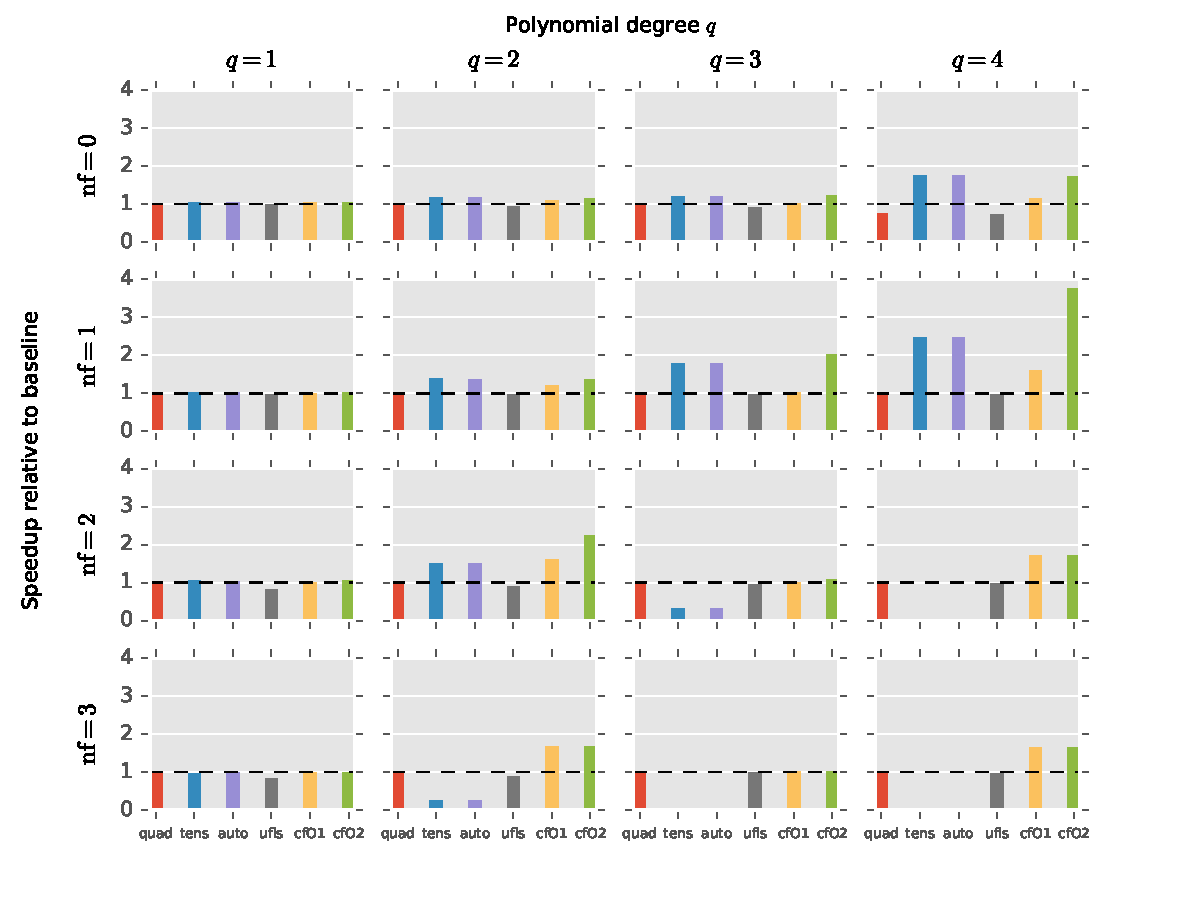
\includegraphics[scale=0.77]{perf-results/mass}}
\caption{Performance evaluation for the \textit{mass} matrix. The bars represent speed-up over the original (unoptimized) code produced by the FEniCS Form Compiler.}\label{fig:mass}
\end{figure}

\begin{figure}
 \makebox[\textwidth][c]{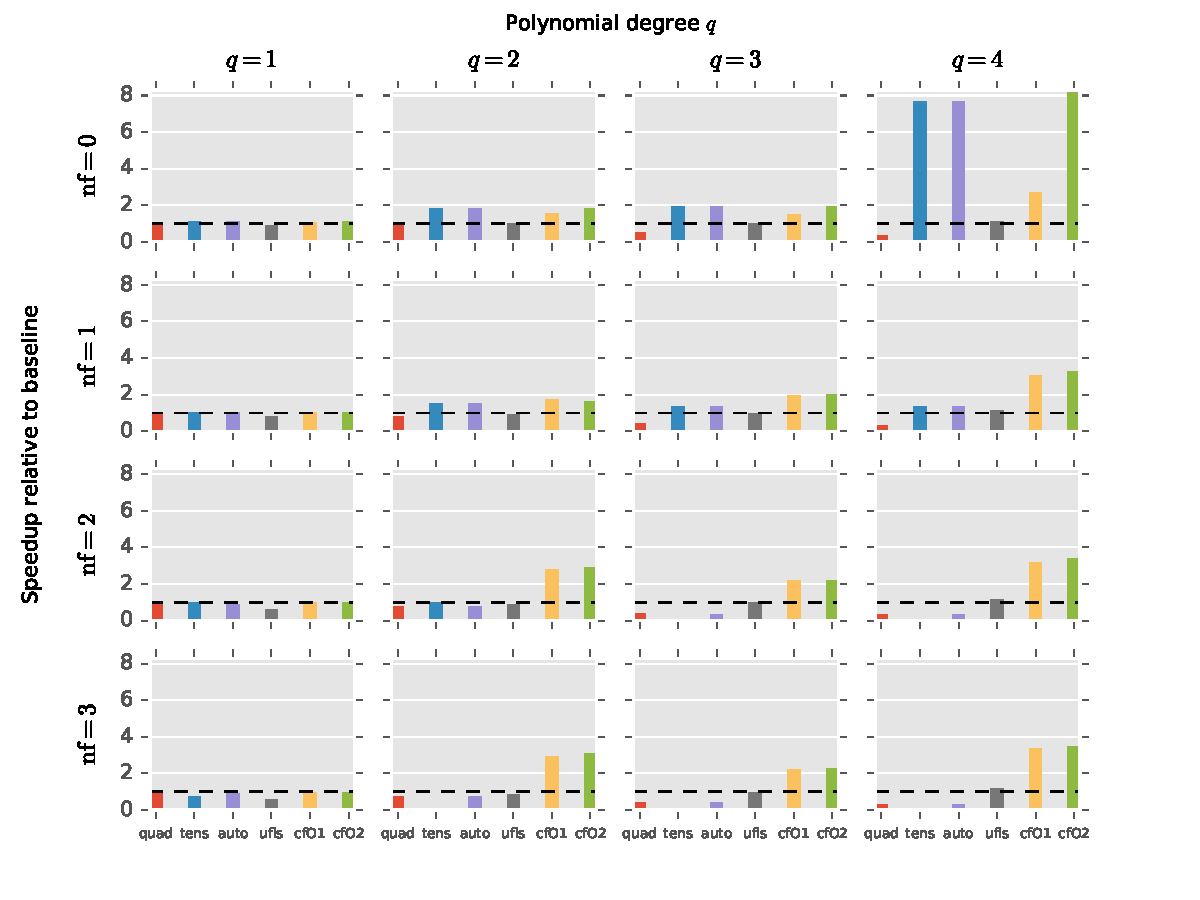
\includegraphics[scale=0.77]{perf-results/helmholtz}}
\caption{Performance evaluation for the bilinear form of a \textit{Helmholtz} equation. The bars represent speed-up over the original (unoptimized) code produced by the FEniCS Form Compiler.}\label{fig:helmholtz}
\end{figure}

\begin{figure}
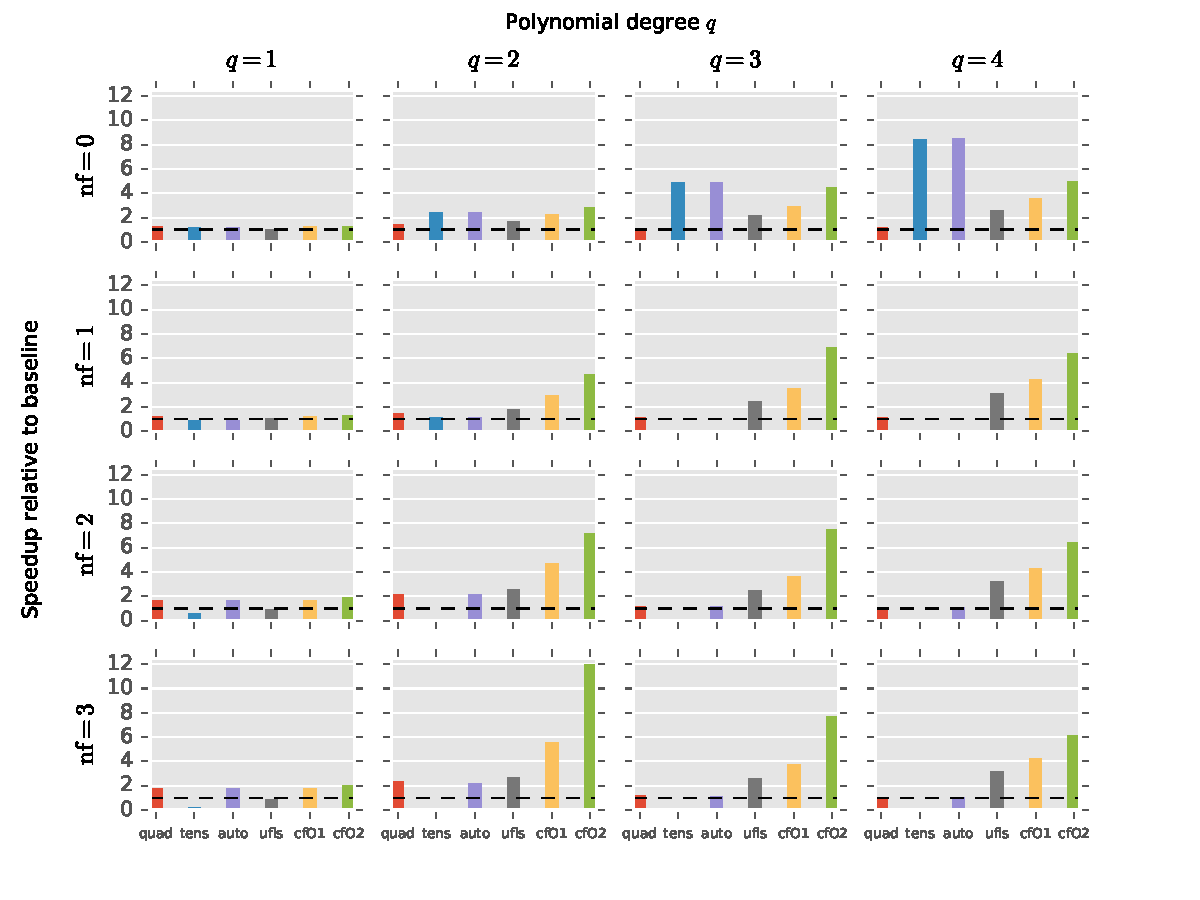
\includegraphics[scale=0.77]{perf-results/elasticity}
\caption{Performance evaluation for the bilinear form arising in an \textit{elastic} model. The bars represent speed-up over the original (unoptimized) code produced by the FEniCS Form Compiler.}\label{fig:elasticity}
\end{figure}

\begin{figure}
 \makebox[\textwidth][c]{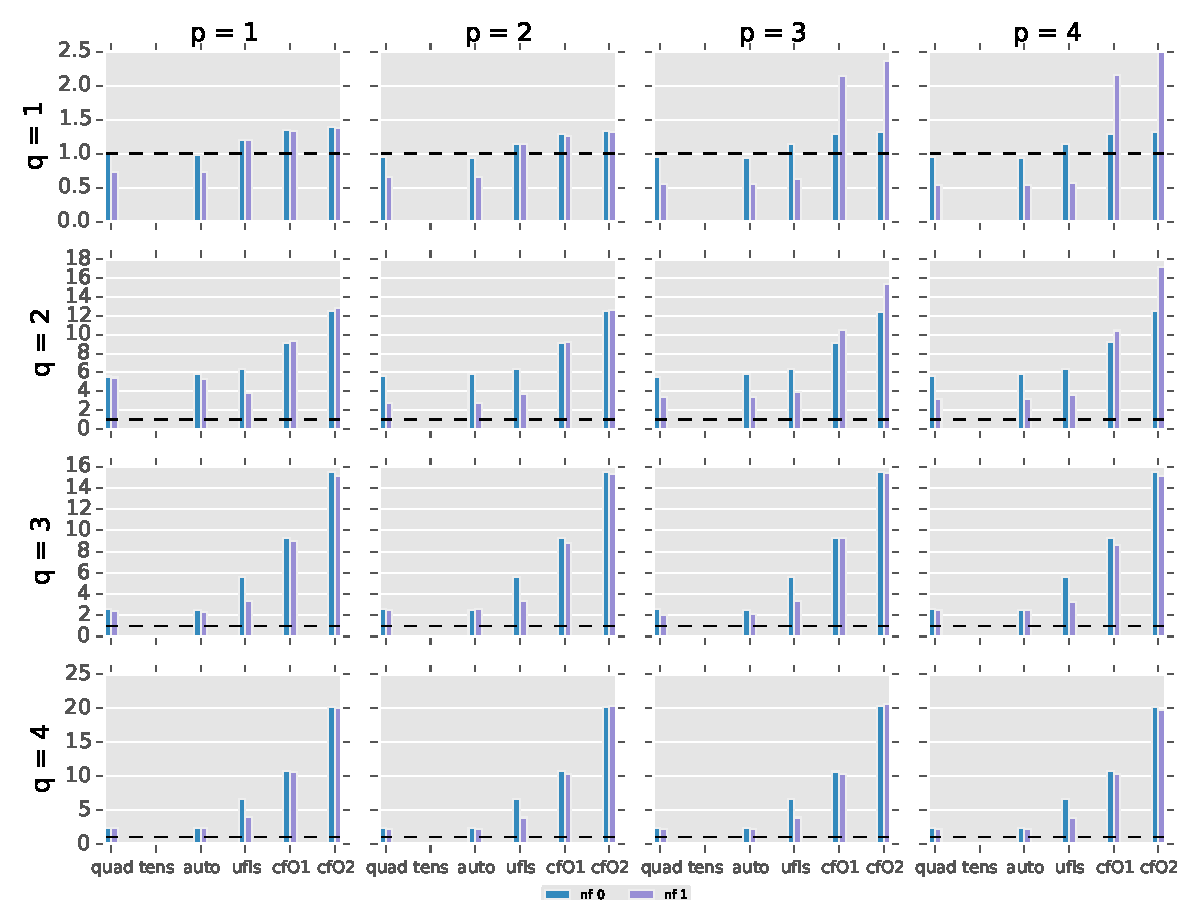
\includegraphics[scale=0.77]{perf-results/hyperelasticity}}
\caption{Performance evaluation for the bilinear form arising in a \textit{hyperelastic} model. The bars represent speed-up over the original (unoptimized) code produced by the FEniCS Form Compiler.}\label{fig:hyperelasticity}
\end{figure}


\paragraph{High level view}
The main observation is that our transformation strategy does not always guarantee minimum execution time. In particular, 5$\%$ of the test cases (3 out of 56, without counting marginal differences) show that \texttt{cfO2} was not optimal in terms of runtime. The most significant of such test cases is the elastic model with $[q=4, nf=0]$. There are two reasons for this. Firstly, low level optimization can have a significant impact on actual performance. For example, the aggressive loop unrolling in \texttt{tens} eliminates operations on zeros and reduces the working set size by not storing entire temporaries; on the other hand, preserving the loop structure can maximize the chances of autovectorization. Secondly, memory constraints are critical, particularly the transformation strategy adpopted when exceeding $T_H$. We will later thoroughly elaborate on all these aspects.

\paragraph{Autovectorization}
The discretizations employed result in inner loops and basis function tables of size multiple of the machine vector length. This, combined with the chosen compilation flags, promotes autovectorization in the majority of code variants. An exception is \texttt{quad} due to the presence of indirection arrays in the generated code. In \texttt{tens}, loop nests are fully unrolled, so the standard loop vectorization is not feasible; manual inspection of the compiled code suggests, however, that block vectorization (\cite{SLP-vect}) is often triggered. In \texttt{ufls}, \texttt{cfO1}, and \texttt{cfO2} the iteration spaces have similar structure (there are a few exceptions in \texttt{cfO2} due to zero-elimination), with loop vectorization being regularly applied, as far as we could evince from compiler reports and manual inspection of assembly code.

\paragraph{Mass}
We start with the simplest of the bilinear forms investigated, the mass matrix. Results are in Figure~\ref{fig:mass}. We first notice that the lack of improvements when $q=1$ is due to the fact that matrix insertion outweighs local assembly. As $q \geq 2$, \texttt{cfO2} generally shows the highest speed-ups. It is worth noting how \texttt{auto} does not always select the fastest implementation: \texttt{auto} always opts for \texttt{tens}, while as $nf \geq 2$ \texttt{quad} would tend to be preferable. On the other hand, \texttt{cfO2} always makes the optimal decision about whether applying pre-evaluation or not.  

\paragraph{Helmholtz}
As happened with the mass matrix problem, when $q=1$ matrix insertion still hides the cost of local assembly. For $q \geq 2$, the general trend is that \texttt{cfO2} outperforms the competitors. In particular, with
\begin{itemize}
\item $nf=0$, the adoption of pre-evaluation by \texttt{cfO2} results in increasingly notable speed-ups over \texttt{cfO1}, as $q$ increases; \texttt{tens} is comparable to \texttt{cfO2}, with \texttt{auto} making the right choice. 
\item $nf=1$, \texttt{auto} picks \texttt{tens}; the choice is however sub-optimal when $q=3$ and $q=4$. This can indirectly be inferred from the large gap between \texttt{cfO1/cfO2} and \texttt{tens/auto}: \texttt{cfO2} applies sharing elimination, but it avoids pre-evaluation. 
\item $nf=2$ and $nf=3$, \texttt{auto} reverts to \texttt{quad}, which would theoretically be the right choice (the flop count is much lower than in \texttt{tens} or what would be produced by pre-evaluation); however, the generated code suffers from the presence of indirection arrays, which break autovectorization and ``traditional'' code motion.
\end{itemize}

The sporadic slow-downs or only marginal improvements exhibited by \texttt{ufls} are imputable to the presence of sharing.

An interesting experiment we performed was relaxing the memory threshold by setting it to $T_H = L3_{size}$. We found that this makes \texttt{cfO2} generally slower as $nf \geq 2$, with a maximum slow-down of 2.16$\times$ with $\langle nf=2, q=2\rangle$. The effects of not having a sensible threshold could even be worse in parallel runs, since the L3 cache is shared by the cores.

\paragraph{Elasticity}
The results for the elastic model are displayed in Figure~\ref{fig:elasticity}. The main observation is that \texttt{cfO2} never triggers pre-evaluation, although in some occasions it should. To clarify this, consider the test case $\langle nf=0, q=2 \rangle$, in which \texttt{tens/auto} show a considerable speed-up over \texttt{cfO2}. \texttt{cfO2} finds pre-evaluation profitable -- that is, actually capable of reducing the operation count -- although it does not apply it because otherwise $T_H$ would be exceeded. However, running the same experiments with $T_H = L3_{size}$ resulted in a dramatic improvement, even higher than that of \texttt{tens}. Our explanation is that despite exceeding $T_H$ by roughly 40$\%$, the save in operation count is so large (5$\times$ in this problem) that pre-evaluation would anyway be the optimal choice. This suggests that our model could be refined to handle the cases in which there is a significant gap between potential cache misses and save in flops.

We also note that:
\begin{itemize}
\item the differences between \texttt{cfO2} and \texttt{cfO1} are due to systematic sharing elimination and the use of symbolic execution to avoid iteration over the zero-valued regions in the basis function tables
\item when $nf=1$, \texttt{auto} prefers \texttt{tens} to \texttt{quad}, which leads to sub-optimal operation counts and execution times
\item \texttt{ufls} generally shows better runtime behaviour than \texttt{quad} and \texttt{tens}. This is due to multiple facts, including avoidance of indirection arrays, preservation of loop structure, a more effective code motion.
\end{itemize}

\paragraph{Hyperelasticity}
In the experiments on the hyperelastic model, shown in Figure~\ref{fig:hyperelasticity}, \texttt{cfO2} exhibits the largest gains out of all problem instances considered in this paper. This is a positive aspect: it means that our transformation algorithm scales with form complexity. The fact that all code transformation systems (apart from \texttt{tens}) show quite significant speed-ups suggests several points. Firstly, the baseline is highly inefficient: with forms as complex as in this hyperelastic model, a trivial translation of integration routines into code should always be avoided since even one of the best general-purpose compilers available (Intel's on an Intel platform at maximum optimization level) is not capable of exploiting the structure inherent in the mathematical expressions generated. Secondly, the code motion strategy really makes a considerable impact. The sharing elimination performed by \texttt{cfO2} in each level of the loop nest ensures a critical reduction in operation count, which results is better execution times. In particular, at higher order, the main difference between \texttt{ufls} and \texttt{cfO2} is due to the application of this transformation to the outer-product loop nest. Clearly, the operation count increases with $q$, and so do the speed-ups. 



\section{Conclusions}
\label{sec:conclusions}
With this research we have set the foundation of optimal finite element integration. We have developed theory and implemented an automated system capable of applying it. The automated system, COFFEE, is integrated in Firedrake, a real-world framework for writing finite element methods. We believe the results are extremely positive. An open problem is understanding how to optimally handle non-linear loop nests. A second open problem is extending our methodology to classes of loops arising in spectral methods; here, the interaction with low level optimization will probably become stronger due to the typically larger working sets deriving from the use of high order function spaces. Lastly, we recall our work is publicly available and is already in use in the latest version of the Firedrake framework.

% Bibliography
\bibliographystyle{ACM-Reference-Format-Journals}
\bibliography{biblio}


\medskip

\end{document}
